\section{Results}
\label{sec:results}

\subsection{Vibe Descriptions Are Maximally Diverse (H1)}

\gptfour produces a unique vibe description for every one of the 497 pages.
Across 18{,}462 total words, we observe 6{,}217 unique word types, yielding a type-token ratio of 0.337.
The mean description length is 254 characters ($\pm$61).
Of the 497 descriptions, 493 (99.2\%) contain the phrase ``it's giving,'' with 33 using the exact lowercase form and the remainder using capitalized or minor variants.
The model consistently employs culturally fluent internet vernacular---terms like ``cottagecore,'' ``main character energy,'' and various ``-core'' suffixes appear naturally throughout the descriptions.

\subsection{Vibe Space Captures Different Information Than Content Space (H2)}

\tabref{tab:clustering} presents clustering comparison results across multiple values of $k$.
The \ari between vibe-space and content-space clusterings ranges from 0.100 to 0.137, indicating that only 10--14\% of page-pair co-cluster assignments agree.
A permutation test at $k{=}10$ yields $p{=}0.0002$, confirming that the observed agreement, while statistically above chance, is very low---vibe space and content space organize pages in fundamentally different ways.

\begin{table}[t]
    \centering
    \caption{Clustering comparison between vibe space and content space across values of $k$. Silhouette scores measure within-space cluster quality~\cite{rousseeuw1987silhouettes}; \ari measures agreement between the two clusterings~\cite{hubert1985ari}. Vibe space consistently achieves higher silhouette scores and low agreement with content space. Best silhouette per row in \textbf{bold}.}
    \begin{tabular}{@{}lccc@{}}
        \toprule
        $k$ & Silhouette (Content) & Silhouette (Vibe) & \ari \\
        \midrule
        5  & 0.033 & \textbf{0.064} & 0.137 \\
        10 & 0.037 & \textbf{0.053} & 0.113 \\
        15 & 0.035 & \textbf{0.060} & 0.103 \\
        20 & 0.037 & \textbf{0.059} & 0.100 \\
        \bottomrule
    \end{tabular}
    \label{tab:clustering}
\end{table}

\subsection{Vibe Space Has Better Cluster Structure (H3)}

Across all values of $k$, vibe-space silhouette scores (0.053--0.064) exceed content-space scores (0.033--0.037).
Bootstrap 95\% confidence intervals at $k{=}10$ are $[0.056, 0.080]$ for vibe space and $[0.046, 0.061]$ for content space.
While both spaces have modest absolute silhouette scores---expected given the diversity of web content---vibe descriptions produce more coherent groupings than raw text.

\subsection{Vibe Space Enables Cross-Domain Discovery (H4)}

\tabref{tab:neighbors} summarizes the nearest-neighbor analysis.
Pages share only 15.1\% of their $K{=}5$ neighbors between the two spaces, compared to 1.0\% expected by chance.
More strikingly, the raw-text cosine similarity of vibe-space neighbors ($0.178 \pm 0.132$) is dramatically lower than that of content-space neighbors ($0.339 \pm 0.087$).
This difference is highly significant (Mann--Whitney $U$, $p < 10^{-6}$) with a very large effect size (Cohen's $d{=}1.44$).

\begin{table}[t]
    \centering
    \caption{Nearest-neighbor analysis ($K{=}5$). Vibe-space neighbors have substantially lower content similarity than content-space neighbors, confirming that vibe space brings together pages from different content domains.}
    \begin{tabular}{@{}lc@{}}
        \toprule
        Metric & Value \\
        \midrule
        Mean neighbor overlap & 0.753 / 5 (15.1\%) \\
        Expected random overlap & 0.050 / 5 (1.0\%) \\
        Content sim.\ of content-space neighbors & $0.339 \pm 0.087$ \\
        Content sim.\ of vibe-space neighbors & $0.178 \pm 0.132$ \\
        Mann--Whitney $U$ $p$-value & $< 10^{-6}$ \\
        Cohen's $d$ & \textbf{1.44} \\
        \bottomrule
    \end{tabular}
    \label{tab:neighbors}
\end{table}

These results confirm that vibe space brings together pages from different content domains that share aesthetic character.
We identify 293 cross-domain page pairs---pages whose vibe-space neighbors have raw-text cosine similarity below 0.15, indicating topically unrelated content.

\subsection{Qualitative Analysis}

\Figref{fig:maps} shows the raw-text and vibe-space UMAP projections side by side.
The vibe map reveals coherent aesthetic regions that cut across topics.
We highlight three illustrative cross-domain clusters:

\para{Early-2010s personal blog energy.}
A Romanian collaboration blog and a British movie review site---different languages, different subjects---cluster together because both project the same warm, hand-crafted, personal-blog aesthetic.

\para{Cozy niche forum energy.}
Gaming forums, tech support forums, and train simulator forums share ``cozy niche forum energy'' despite wildly different content.
The vibe captures the community format, conversational tone, and retro web design rather than the subject matter.

\para{Corporate LinkedIn energy.}
Pages about corporate acquisitions, academic engineering programs, and professional development services cluster together, unified by polished, institutional communication style.

\begin{figure}[t]
    \centering
    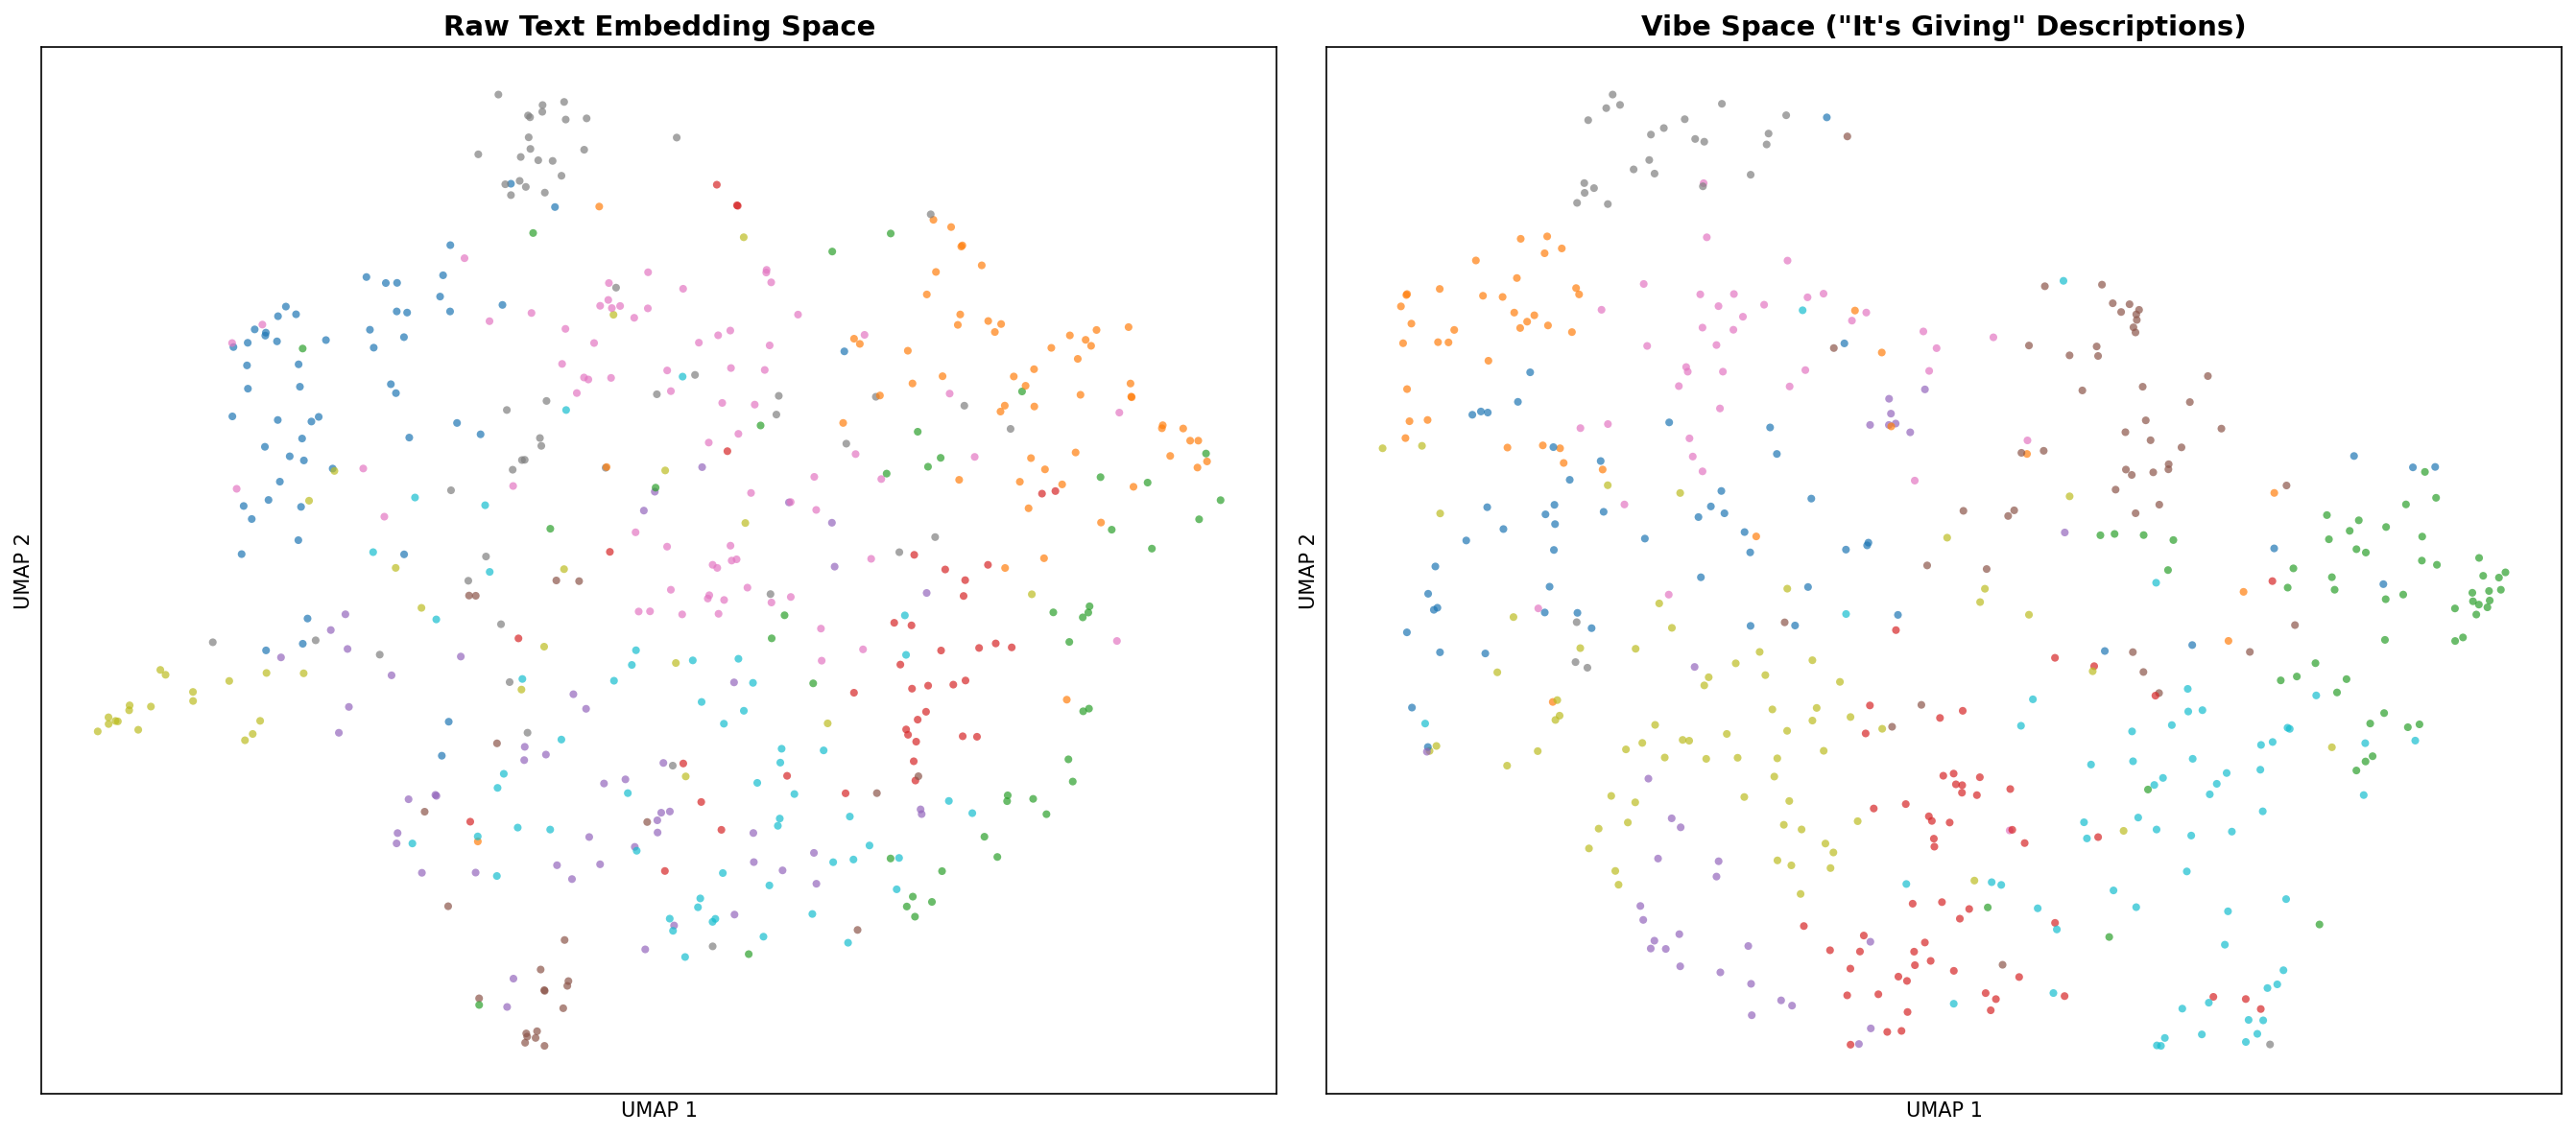
\includegraphics[width=0.95\linewidth]{figures/raw_vs_vibe_space.png}
    \caption{UMAP projections of 497 web pages in content space \figleft and vibe space \figright. Points are colored by content-space cluster assignment in both panels. The rearrangement of colors in the right panel confirms that vibe space organizes pages differently from content space.}
    \label{fig:maps}
\end{figure}

\subsection{Dimensionality Analysis}

Vibe embeddings require 128 principal components to explain 90\% of variance, compared to 178 for raw-text embeddings.
Vibe space is more compact, suggesting that aesthetic character occupies a lower-dimensional manifold than topical content---there are fewer ``vibe dimensions'' than ``topic dimensions.''
